% Options for packages loaded elsewhere
% Options for packages loaded elsewhere
\PassOptionsToPackage{unicode}{hyperref}
\PassOptionsToPackage{hyphens}{url}
%
\documentclass[
  ignorenonframetext,
]{beamer}
\newif\ifbibliography
\usepackage{pgfpages}
\setbeamertemplate{caption}[numbered]
\setbeamertemplate{caption label separator}{: }
\setbeamercolor{caption name}{fg=normal text.fg}
\beamertemplatenavigationsymbolsempty
% remove section numbering
\setbeamertemplate{part page}{
  \centering
  \begin{beamercolorbox}[sep=16pt,center]{part title}
    \usebeamerfont{part title}\insertpart\par
  \end{beamercolorbox}
}
\setbeamertemplate{section page}{
  \centering
  \begin{beamercolorbox}[sep=12pt,center]{section title}
    \usebeamerfont{section title}\insertsection\par
  \end{beamercolorbox}
}
\setbeamertemplate{subsection page}{
  \centering
  \begin{beamercolorbox}[sep=8pt,center]{subsection title}
    \usebeamerfont{subsection title}\insertsubsection\par
  \end{beamercolorbox}
}
% Prevent slide breaks in the middle of a paragraph
\widowpenalties 1 10000
\raggedbottom
\AtBeginPart{
  \frame{\partpage}
}
\AtBeginSection{
  \ifbibliography
  \else
    \frame{\sectionpage}
  \fi
}
\AtBeginSubsection{
  \frame{\subsectionpage}
}
\usepackage{iftex}
\ifPDFTeX
  \usepackage[T1]{fontenc}
  \usepackage[utf8]{inputenc}
  \usepackage{textcomp} % provide euro and other symbols
\else % if luatex or xetex
  \usepackage{unicode-math} % this also loads fontspec
  \defaultfontfeatures{Scale=MatchLowercase}
  \defaultfontfeatures[\rmfamily]{Ligatures=TeX,Scale=1}
\fi
\usepackage{lmodern}

\ifPDFTeX\else
  % xetex/luatex font selection
\fi
% Use upquote if available, for straight quotes in verbatim environments
\IfFileExists{upquote.sty}{\usepackage{upquote}}{}
\IfFileExists{microtype.sty}{% use microtype if available
  \usepackage[]{microtype}
  \UseMicrotypeSet[protrusion]{basicmath} % disable protrusion for tt fonts
}{}
\makeatletter
\@ifundefined{KOMAClassName}{% if non-KOMA class
  \IfFileExists{parskip.sty}{%
    \usepackage{parskip}
  }{% else
    \setlength{\parindent}{0pt}
    \setlength{\parskip}{6pt plus 2pt minus 1pt}}
}{% if KOMA class
  \KOMAoptions{parskip=half}}
\makeatother


\usepackage{longtable,booktabs,array}
\usepackage{calc} % for calculating minipage widths
\usepackage{caption}
% Make caption package work with longtable
\makeatletter
\def\fnum@table{\tablename~\thetable}
\makeatother
\usepackage{graphicx}
\makeatletter
\newsavebox\pandoc@box
\newcommand*\pandocbounded[1]{% scales image to fit in text height/width
  \sbox\pandoc@box{#1}%
  \Gscale@div\@tempa{\textheight}{\dimexpr\ht\pandoc@box+\dp\pandoc@box\relax}%
  \Gscale@div\@tempb{\linewidth}{\wd\pandoc@box}%
  \ifdim\@tempb\p@<\@tempa\p@\let\@tempa\@tempb\fi% select the smaller of both
  \ifdim\@tempa\p@<\p@\scalebox{\@tempa}{\usebox\pandoc@box}%
  \else\usebox{\pandoc@box}%
  \fi%
}
% Set default figure placement to htbp
\def\fps@figure{htbp}
\makeatother





\setlength{\emergencystretch}{3em} % prevent overfull lines

\providecommand{\tightlist}{%
  \setlength{\itemsep}{0pt}\setlength{\parskip}{0pt}}



 


\makeatletter
\@ifpackageloaded{caption}{}{\usepackage{caption}}
\AtBeginDocument{%
\ifdefined\contentsname
  \renewcommand*\contentsname{Table of contents}
\else
  \newcommand\contentsname{Table of contents}
\fi
\ifdefined\listfigurename
  \renewcommand*\listfigurename{List of Figures}
\else
  \newcommand\listfigurename{List of Figures}
\fi
\ifdefined\listtablename
  \renewcommand*\listtablename{List of Tables}
\else
  \newcommand\listtablename{List of Tables}
\fi
\ifdefined\figurename
  \renewcommand*\figurename{Figure}
\else
  \newcommand\figurename{Figure}
\fi
\ifdefined\tablename
  \renewcommand*\tablename{Table}
\else
  \newcommand\tablename{Table}
\fi
}
\@ifpackageloaded{float}{}{\usepackage{float}}
\floatstyle{ruled}
\@ifundefined{c@chapter}{\newfloat{codelisting}{h}{lop}}{\newfloat{codelisting}{h}{lop}[chapter]}
\floatname{codelisting}{Listing}
\newcommand*\listoflistings{\listof{codelisting}{List of Listings}}
\makeatother
\makeatletter
\makeatother
\makeatletter
\@ifpackageloaded{caption}{}{\usepackage{caption}}
\@ifpackageloaded{subcaption}{}{\usepackage{subcaption}}
\makeatother

\usepackage{bookmark}
\IfFileExists{xurl.sty}{\usepackage{xurl}}{} % add URL line breaks if available
\urlstyle{same}
\hypersetup{
  pdftitle={NexusOS},
  pdfauthor={张家文},
  hidelinks,
  pdfcreator={LaTeX via pandoc}}


\title{NexusOS}
\author{张家文}
\date{}

\begin{document}
\frame{\titlepage}


\begin{frame}{NexusOS}
\phantomsection\label{nexusos}
基于 Rust 的多核、异步、\textbf{框内核 (Framekernel)} 架构的操作系统。
\end{frame}

\begin{frame}
\begin{block}{架构:框内核 (Framekernel) - 核心思想}
\phantomsection\label{ux67b6ux6784ux6846ux5185ux6838-framekernel---ux6838ux5fc3ux601dux60f3}
\begin{quote}
融合''微内核的安全性''与''单体内核的性能''的新型操作系统架构。
\end{quote}

\begin{itemize}
\tightlist
\item
  \textbf{单地址空间}:
  内核态所有组件共享同一地址空间,通过函数调用高效通信。
\end{itemize}
\end{block}
\end{frame}

\begin{frame}[fragile]
\begin{itemize}
\tightlist
\item
  \textbf{Rust 全栈实现,分区保证安全}:

  \begin{itemize}
  \tightlist
  \item
    \textbf{OS Framework (框架)}: 极少量 \texttt{unsafe}
    代码,封装硬件操作为安全 API。
  \item
    \textbf{OS Services (服务)}: 只能用 \texttt{safe\ Rust}
    编写,实现绝大部分内核功能。
  \end{itemize}
\item
  \textbf{最小化可信基 (TCB)}: 系统的内存安全仅依赖于体量很小的 OS
  Framework。
\end{itemize}
\end{frame}

\begin{frame}[fragile]
\begin{block}{架构:框内核的设计要求}
\phantomsection\label{ux67b6ux6784ux6846ux5185ux6838ux7684ux8bbeux8ba1ux8981ux6c42}
\begin{itemize}
\tightlist
\item
  \textbf{Soundness (健全性)}: 框架提供的安全 API
  应保证使用者无法触发未定义行为。
\item
  \textbf{Expressiveness (表达力)}: API 需足够强大,使开发者能在
  \texttt{safe\ Rust} 中实现绝大多数 OS 功能。
\item
  \textbf{Minimalism (极简性)}: 框架体量越小越好,功能尽可能外置。
\item
  \textbf{Efficiency (高效性)}: API 应为零开销或仅引入极小的开销。
\end{itemize}
\end{block}
\end{frame}

\begin{frame}
\begin{block}{异步与同步的区别}
\phantomsection\label{ux5f02ux6b65ux4e0eux540cux6b65ux7684ux533aux522b}
内核异步化的关键点之一是内核控制流的隔离与切换
\end{block}
\end{frame}

\begin{frame}
\begin{block}{内核控制流的隔离}
\phantomsection\label{ux5185ux6838ux63a7ux5236ux6d41ux7684ux9694ux79bb}
同步时,内核控制流是通过多个内核栈以及存储的寄存器值来隔离的。

异步时,内核控制流通过future自动生成的状态机来隔离。
\end{block}
\end{frame}

\begin{frame}[fragile]
\begin{block}{内核控制流的切换}
\phantomsection\label{ux5185ux6838ux63a7ux5236ux6d41ux7684ux5207ux6362}
同步时,内核控制流通过切换内核栈和寄存器的值(即\texttt{context\_switch}函数)来切换。

异步时,内核控制流通过切换状态机来切换。或者是通过\texttt{future::poll}函数来切换。
\end{block}
\end{frame}

\begin{frame}
\begin{block}{对于实现的影响}
\phantomsection\label{ux5bf9ux4e8eux5b9eux73b0ux7684ux5f71ux54cd}
同步时, 1. 内核任务需要分配独立的内核栈, 2.
并且需要保存和恢复寄存器的值,即需要task\_context字段来保存和恢复寄存器的值
\end{block}
\end{frame}

\begin{frame}[fragile]
异步时, 1. 内核任务则不需要独立的内核栈, 2.
无需保存和恢复寄存器,不需要task\_context字段(对于内核线程与用户线程的切换来说,相应的寄存器数据保存到每个cpu都有的内核栈中即可,不需要单独用task\_context字段来保存)

\begin{enumerate}
\setcounter{enumi}{2}
\tightlist
\item
  没有显式的任务切换(即没有显式的context\_switch函数,而是可能在某一个
  await
  点切换),且此时一个内核任务对应一个future状态机,所以可以把运行的任务存到相应的future状态机中(通过将要运行的任务作为async
  函数的参数或 async 闭包的捕获变量,然后把spawn此future)。
\end{enumerate}

\begin{block}{进程模型:核心理念 - 异步与解耦}
\phantomsection\label{ux8fdbux7a0bux6a21ux578bux6838ux5fc3ux7406ux5ff5---ux5f02ux6b65ux4e0eux89e3ux8026}
\begin{itemize}
\tightlist
\item
  \textbf{解耦}: \textbf{可调度实体 (Task)} 与 \textbf{进程语义
  (ThreadGroup)} 分离。
\item
  \textbf{异步化}:

  \begin{itemize}
  \tightlist
  \item
    内核控制流由 \texttt{Future} 状态机隔离与切换。
  \item
    抛弃了传统的独立内核栈与显式上下文切换 (\texttt{context\_switch})。
  \end{itemize}
\end{itemize}
\end{block}
\end{frame}

\begin{frame}
\begin{block}{进程模型:核心理念 - 状态隔离}
\phantomsection\label{ux8fdbux7a0bux6a21ux578bux6838ux5fc3ux7406ux5ff5---ux72b6ux6001ux9694ux79bb}
\begin{itemize}
\tightlist
\item
  \textbf{信息与状态分离}:

  \begin{itemize}
  \tightlist
  \item
    \textbf{信息 (ThreadSharedInfo)}: 对外共享,可被其他任务观测。
  \item
    \textbf{状态 (ThreadState)}: 对内私有,仅任务自身访问。
  \end{itemize}
\end{itemize}
\end{block}
\end{frame}

\begin{frame}[fragile]
\begin{block}{进程模型:关键数据结构}
\phantomsection\label{ux8fdbux7a0bux6a21ux578bux5173ux952eux6570ux636eux7ed3ux6784}
\begin{longtable}[]{@{}
  >{\raggedright\arraybackslash}p{(\linewidth - 2\tabcolsep) * \real{0.5000}}
  >{\raggedright\arraybackslash}p{(\linewidth - 2\tabcolsep) * \real{0.5000}}@{}}
\toprule\noalign{}
\begin{minipage}[b]{\linewidth}\raggedright
结构
\end{minipage} & \begin{minipage}[b]{\linewidth}\raggedright
作用
\end{minipage} \\
\midrule\noalign{}
\endhead
\texttt{Task} & 纯调度实体,内核异步运行的最小单元。 \\
\texttt{ThreadGroup} & 用户态所见的''进程'',管理一组
Task,共享资源。 \\
\texttt{ThreadState} &
\textbf{系统调用的''工作集''},聚合了任务运行所需的所有资源。 \\
\bottomrule\noalign{}
\end{longtable}
\end{block}
\end{frame}

\begin{frame}[fragile]
\texttt{ThreadSharedInfo} \textbar{} 记录
TID、亲缘关系、生命周期等可被其他线程观测的\textbf{共享状态}。\textbar{}\\
\texttt{Lifecycle} \textbar{} 原子状态机,管理线程生命周期(如 Running,
Zombie)与退出等待。 \textbar{}
\end{frame}

\begin{frame}[fragile]
\begin{block}{VFS 设计:整体架构}
\phantomsection\label{vfs-ux8bbeux8ba1ux6574ux4f53ux67b6ux6784}
\begin{itemize}
\tightlist
\item
  \textbf{目标}: 纯异步、高性能、易扩展的虚拟文件系统。
\item
  \textbf{特点}:

  \begin{itemize}
  \tightlist
  \item
    \textbf{全异步接口}: 所有文件操作均返回 \texttt{Future}。
  \item
    \textbf{静态分发}: 避免 \texttt{dyn\ Trait} 开销,使用 \texttt{enum}
    在编译期确定调用路径。
  \item
    \textbf{分层设计}: 系统调用适配层、VFS 核心层、具体文件系统实现层。
  \end{itemize}
\end{itemize}
\end{block}
\end{frame}

\begin{frame}
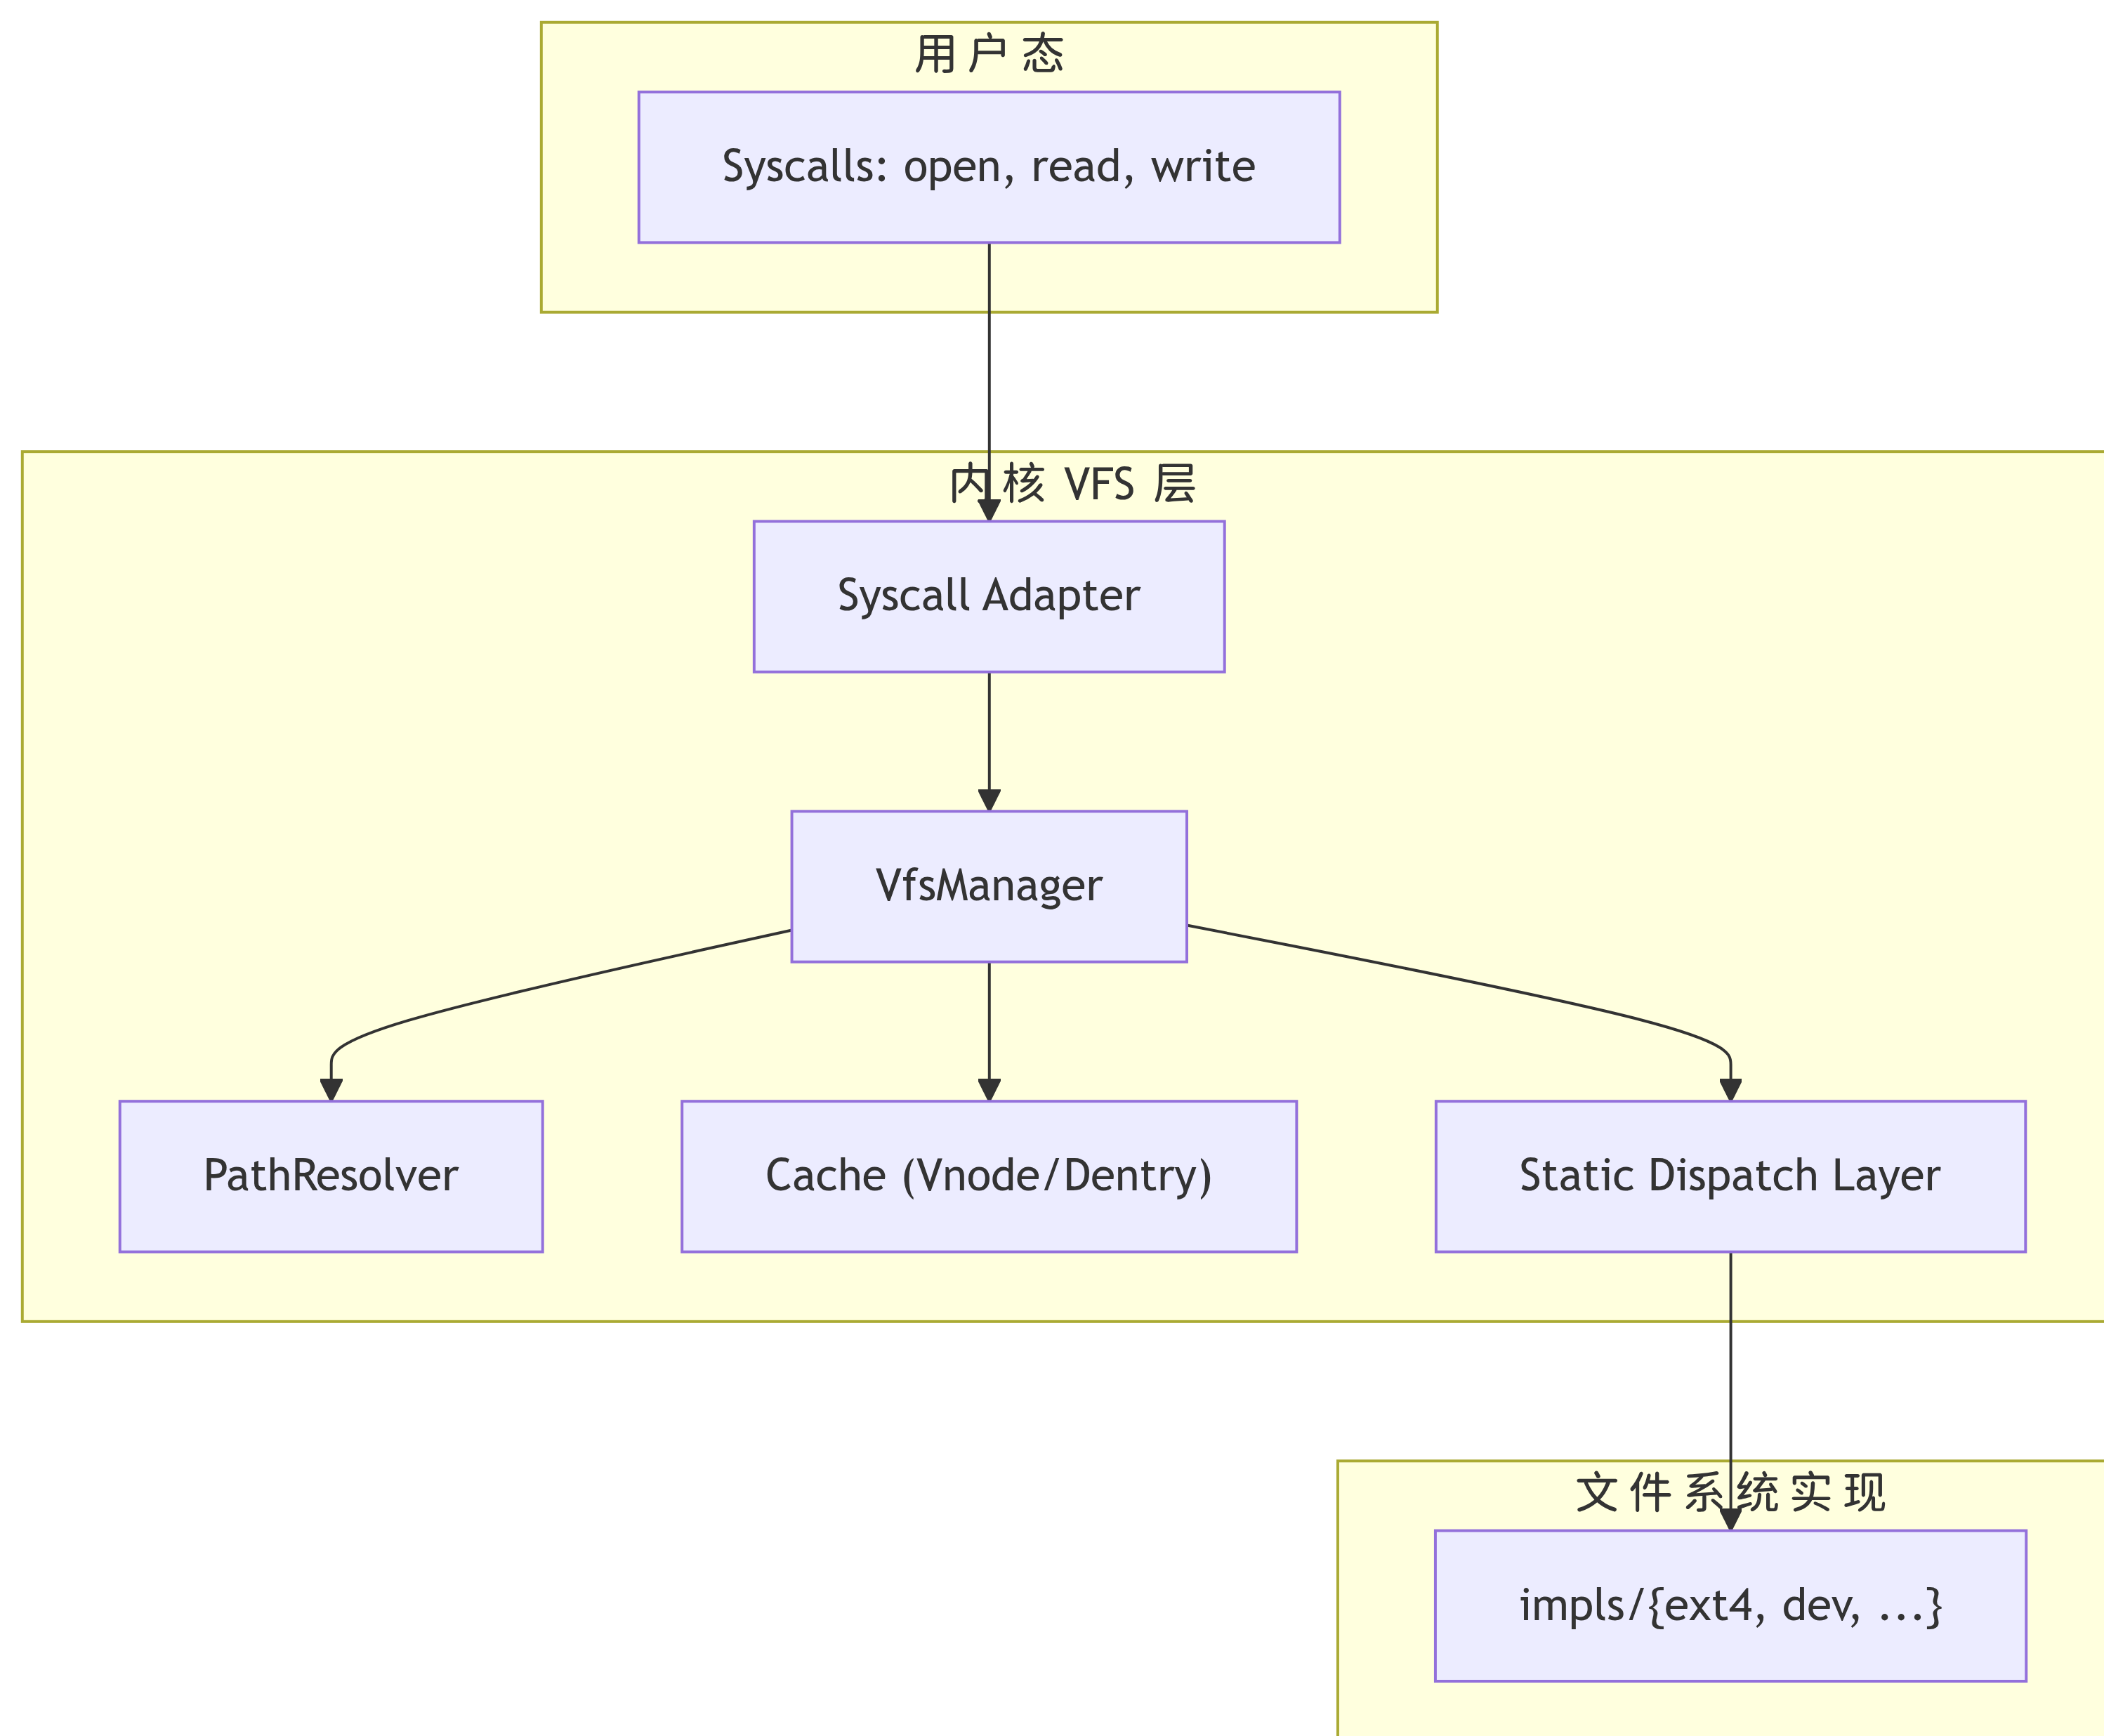
\includegraphics[width=8.02in,height=6.63in]{slide_files/figure-beamer/mermaid-figure-1.png}
\end{frame}

\begin{frame}[fragile]
\begin{block}{内存管理:基于 Asterinas}
\phantomsection\label{ux5185ux5b58ux7ba1ux7406ux57faux4e8e-asterinas}
\begin{itemize}
\tightlist
\item
  \textbf{模型来源}: 完全沿用
  \href{https://github.com/asterinas/asterinas}{Asterinas}
  的安全内存模型。
\item
  \textbf{设计目标}:
  在单地址空间内实现内核特权分离,提供强大的内存安全保障。
\item
  \textbf{核心组件}:

  \begin{itemize}
  \tightlist
  \item
    \textbf{物理内存管理}: \texttt{buddy\_system\_allocator} +
    \texttt{Frame} 抽象。
  \item
    \textbf{元数据系统}: \texttt{MetaSlot} 将物理帧与元数据 O(1)
    映射,支持 RTTI。
  \item
    \textbf{虚拟内存}: \texttt{Vmar} (虚拟内存区域) 与
    \texttt{VmMapping} 精细化管理地址空间。
  \end{itemize}
\end{itemize}
\end{block}
\end{frame}

\begin{frame}
\begin{block}{内存管理:关键抽象}
\phantomsection\label{ux5185ux5b58ux7ba1ux7406ux5173ux952eux62bdux8c61}
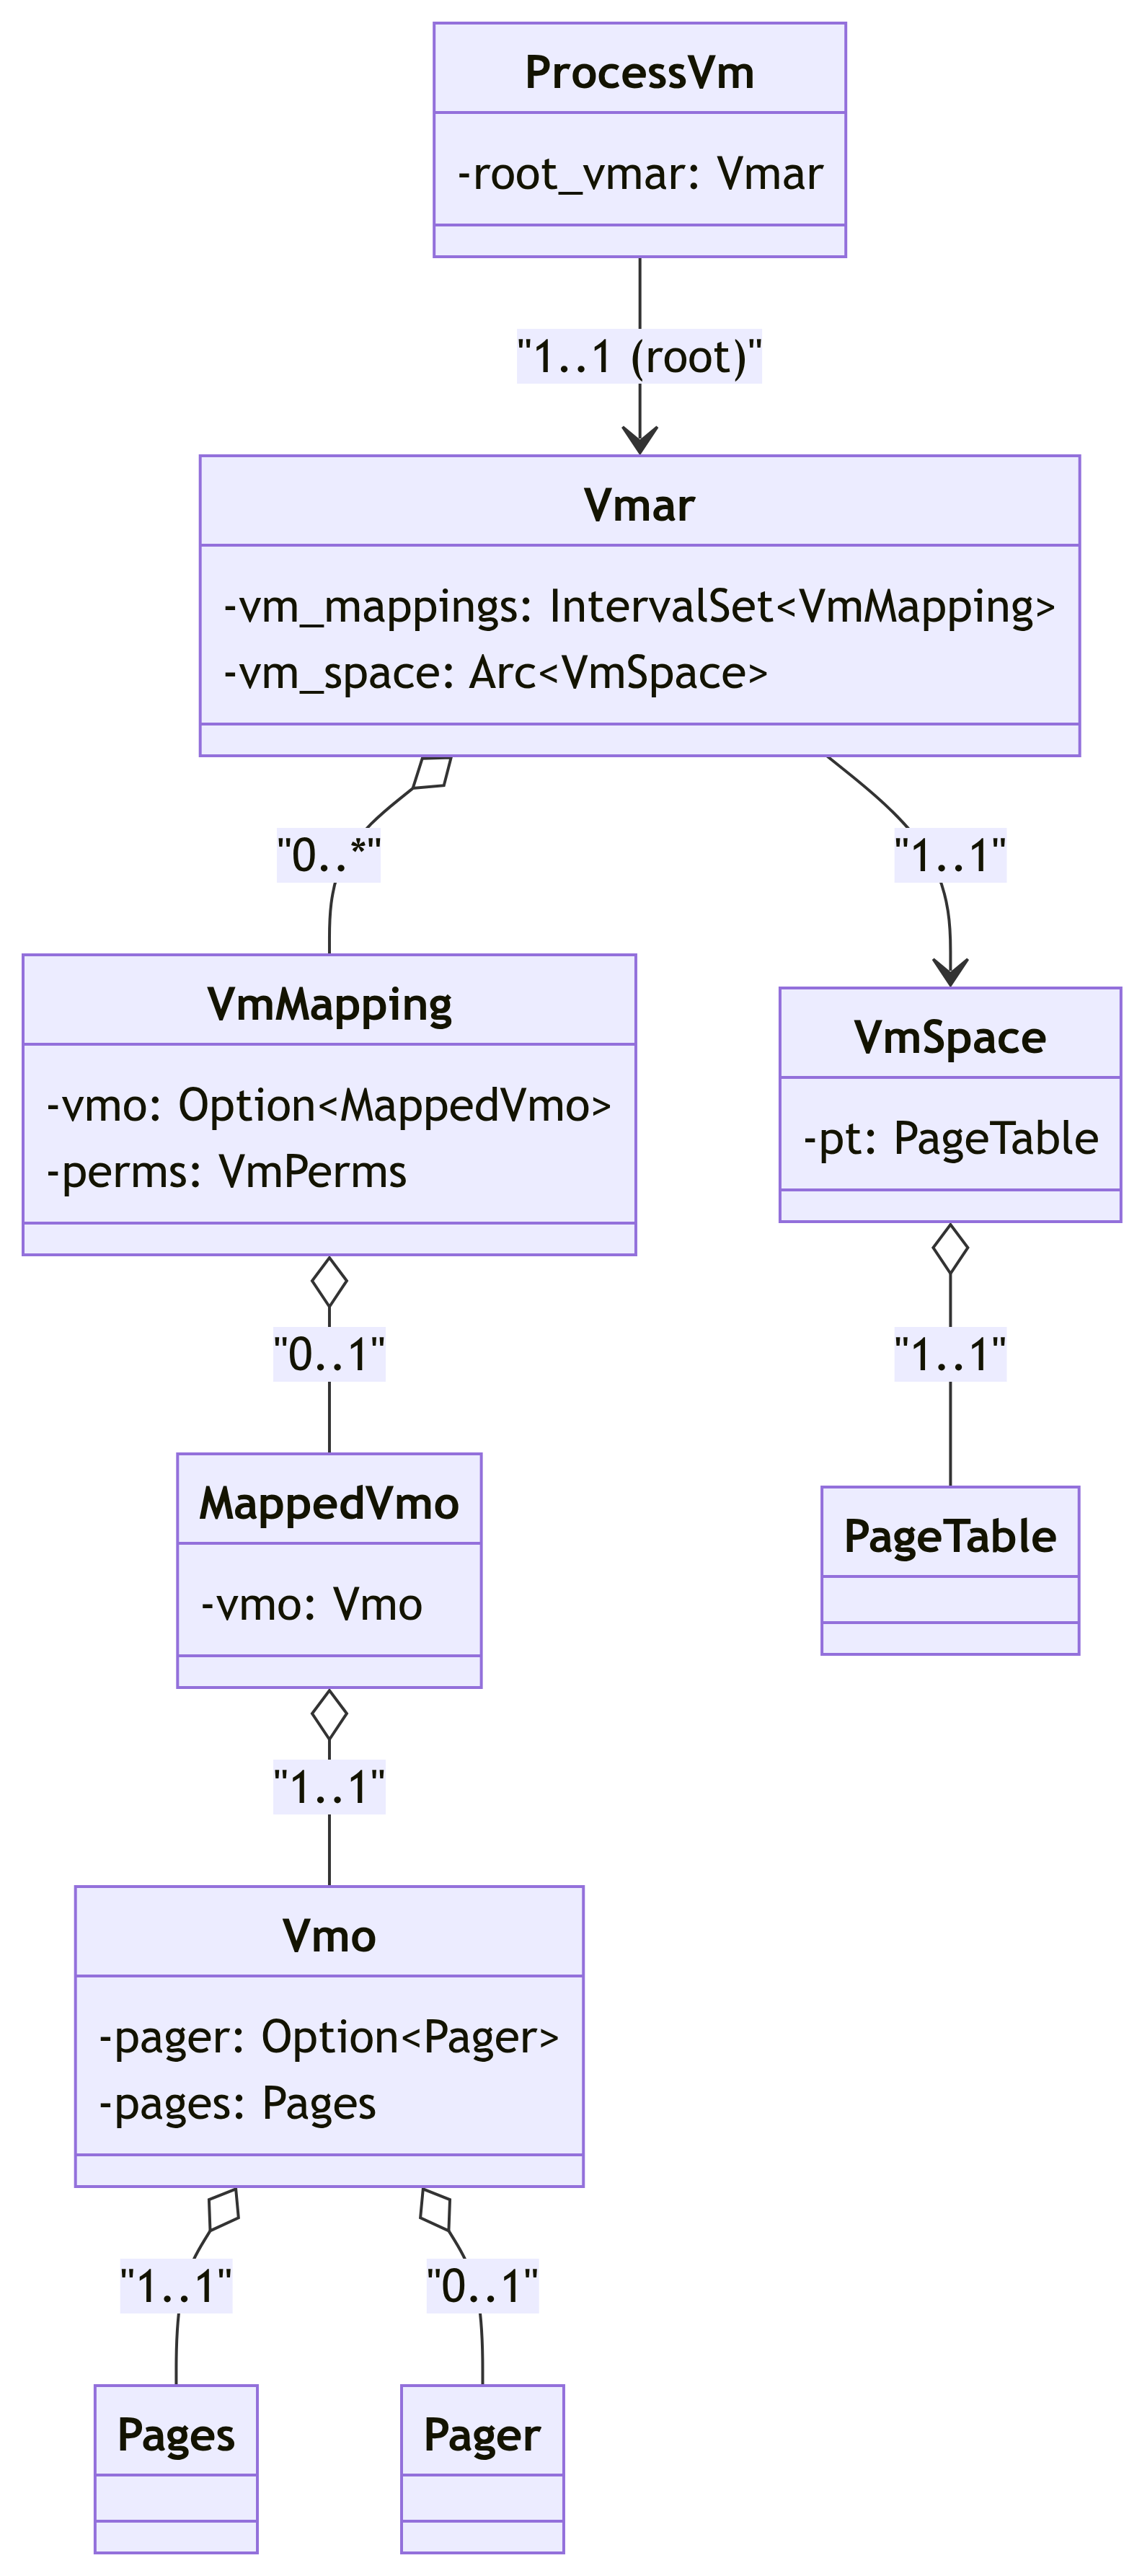
\includegraphics[width=4.13in,height=9.3in]{slide_files/figure-beamer/mermaid-figure-2.png}
\end{block}
\end{frame}

\begin{frame}[fragile]
\begin{block}{核心特性}
\phantomsection\label{ux6838ux5fc3ux7279ux6027}
\begin{itemize}
\tightlist
\item
  \textbf{SMP 与异步化改造}:

  \begin{itemize}
  \tightlist
  \item
    完整的 RISC-V 多核启动流程 (BSP+AP)。
  \item
    引入 \texttt{maitake} 异步调度器,内核由 \texttt{Future} 驱动。
  \item
    实现了高效、类型安全的核间中断 (IPI) 机制。
  \end{itemize}
\item
  \textbf{分层错误处理}:

  \begin{itemize}
  \tightlist
  \item
    基于 \texttt{error-stack} 构建带丰富上下文的内部错误报告。
  \item
    在 VFS 等模块边界,将内部错误转换为统一的 \texttt{Errno}。
  \item
    轻量化设计,对正常执行路径性能影响极小。
  \end{itemize}
\end{itemize}
\end{block}
\end{frame}

\begin{frame}[fragile]
\begin{block}{挑战与对策}
\phantomsection\label{ux6311ux6218ux4e0eux5bf9ux7b56}
\begin{itemize}
\tightlist
\item
  \textbf{地址混淆}: AP 启动时,误用虚拟地址而非物理地址。

  \begin{itemize}
  \tightlist
  \item
    \textbf{对策}: 严格区分地址空间,向固件传递物理地址。
  \end{itemize}
\item
  \textbf{初始化依赖}: \texttt{timer} 初始化依赖尚未就绪的 \texttt{smp}
  IPI。

  \begin{itemize}
  \tightlist
  \item
    \textbf{对策}: 调整模块加载顺序,显式化依赖。
  \end{itemize}
\item
  \textbf{获取当前任务}: 异步模型下,无法用全局变量追踪
  \texttt{current\_task}。

  \begin{itemize}
  \tightlist
  \item
    \textbf{对策}: 扩展调度器 \texttt{Task} 元数据,从中安全获取。
  \end{itemize}
\end{itemize}
\end{block}
\end{frame}

\begin{frame}{Q \& A}
\phantomsection\label{q-a}
Thanks!
\end{frame}




\end{document}
